\section{Work and Energy}

\subsection{\red{Energy}}
\blue{Mostly complete in "Energy and work".}

\noindent \red{Add information as shown in Fig \ref{fig:Energy}. Equations of potential gravitational and elastic are already included in reference page}

\begin{figure}[h!]
    \centering 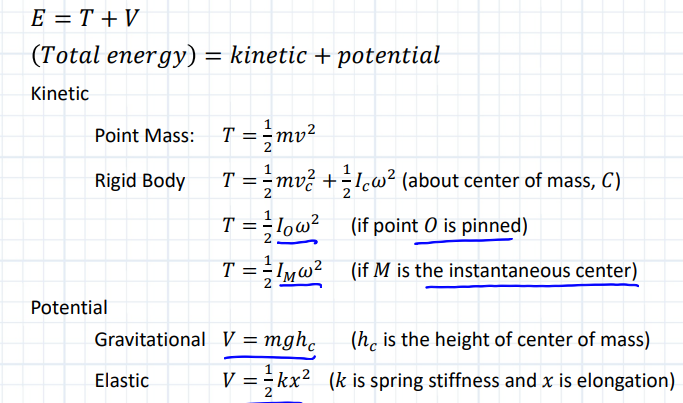
\includegraphics[width=0.8\textwidth]{WorkEnergyFigs/Energy.png}
    \caption{From L29-Notes, Slide 8}
    \label{fig:Energy}
\end{figure}

\subsection{Work}
    \subsubsection{\red{Work-Energy}}
    \red{Include equation and description shown in Fig \ref{fig:WorkEnergy}}
    \begin{figure}[h!]
    \centering 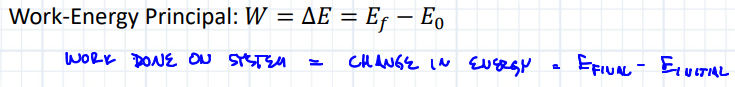
\includegraphics[width=0.8\textwidth]{WorkEnergyFigs/WorkEnergy.png}
    \caption{From L29-Notes, Slide 9}
    \label{fig:WorkEnergy}
\end{figure}

    \subsubsection{\red{Work done by a Force}}
    \blue{Complete in "Energy and work"}

    \noindent \red{Include example shown in Fig \ref{fig:WorkExample}}
    \begin{figure}[h!]
    \centering 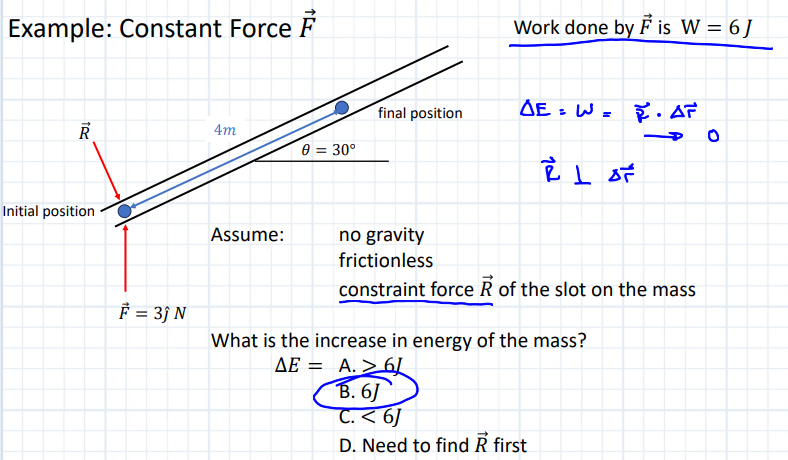
\includegraphics[width=0.85\textwidth]{WorkEnergyFigs/WorkExample.png}
    \caption{From L30-Notes, slide 6}
    \label{fig:WorkExample}
\end{figure}

    \subsubsection{Conservative vs Non-conservative forces}
    \blue{Complete in "Energy and work"}

    \subsubsection{\red{Work done by Friction}}
    \red{Add information and example shown in Fig \ref{fig:WorkFriction}}
    \begin{figure}[h!]
    \centering 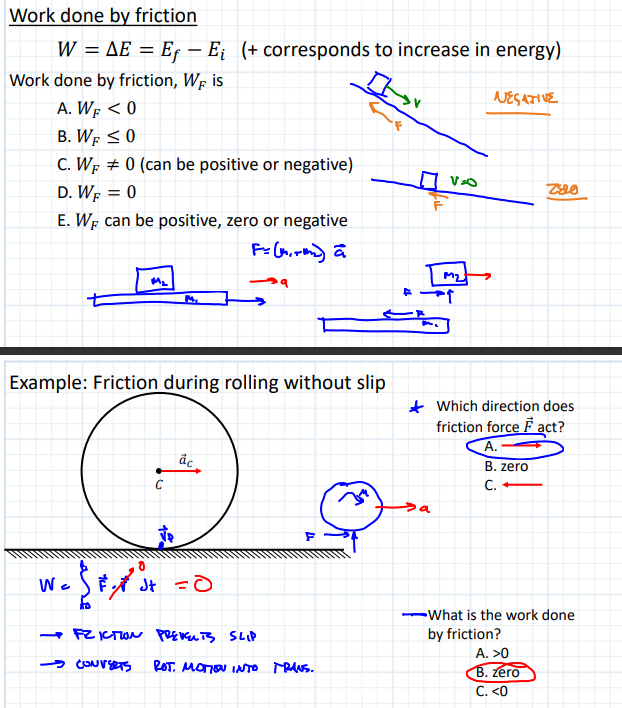
\includegraphics[width=0.85\textwidth]{WorkEnergyFigs/WorkFriction.png}
    \caption{From L30-Notes, slides 11-12}
    \label{fig:WorkFriction}
    \end{figure}
    
    \subsubsection{\red{Work done by a Moment}}
    \red{Add information and example shown in Fig \ref{fig:WorkMoment}}
    
    \begin{figure}[h!]
    \centering 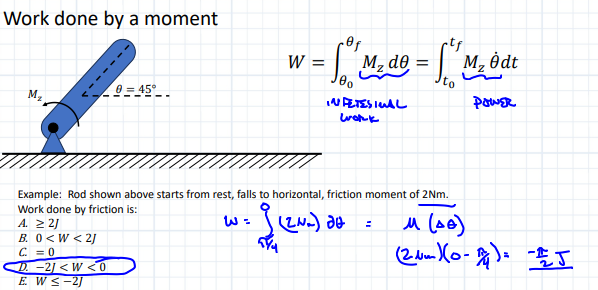
\includegraphics[width=0.85\textwidth]{WorkEnergyFigs/WorkMoment.png}
    \caption{From L30-Notes, slide 13}
    \label{fig:WorkMoment}
    \end{figure}
    
\subsection{Friction}
    \subsubsection{Stick, Transition, Slip}
    \red{Add information shown in Fig \ref{fig:Friction}}
    
    \begin{figure}[h!]
    \centering 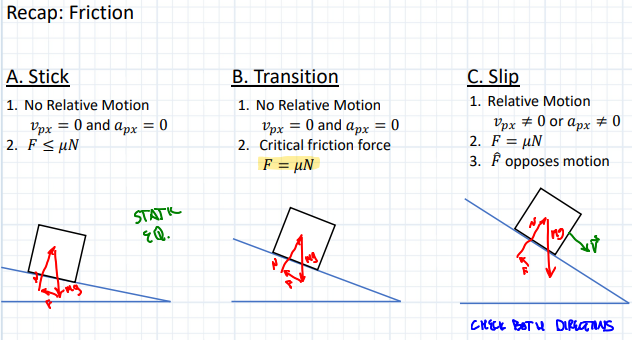
\includegraphics[width=0.85\textwidth]{WorkEnergyFigs/Friction.png}
    \caption{From L33-Notes, slide 2}
    \label{fig:Friction}
    \end{figure}
    
    \subsubsection{Solution procedure}
    \red{Add information shown in Fig \ref{fig:FrictionSolutionProcedure}}
    
    \begin{figure}[h!]
    \centering 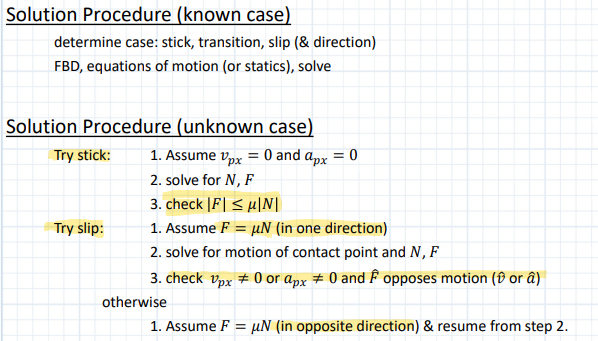
\includegraphics[width=0.85\textwidth]{WorkEnergyFigs/FrictionSolutionProcedure.png}
    \caption{From L30-Notes, slide 13}
    \label{fig:FrictionSolutionProcedure}
    \end{figure}

\subsection{\red{Momentum}}
\red{Add short summary like in Fig \ref{fig:Momentum} at the end of the section}
    \begin{figure}[h!]
    \centering 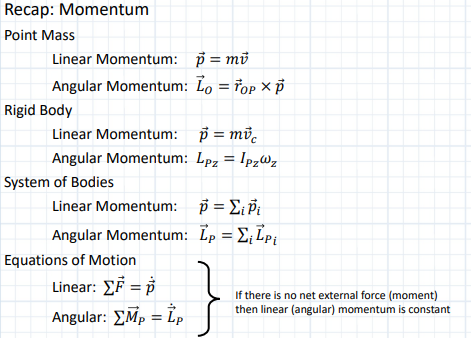
\includegraphics[width=0.85\textwidth]{WorkEnergyFigs/Momentum.png}
    \caption{From L31-Notes, slide 11}
    \label{fig:Momentum}
    \end{figure}
    
    \subsubsection{of a point mass}
    \blue{Complete in "Momentum, impulse and collisions"}
    
    \subsubsection{of a rigid body}
    \blue{Complete in "Momentum, impulse and collisions"}
    
    \subsubsection{of a system of rigid bodies}
    \blue{Complete in "Momentum, impulse and collisions"}

\subsection{Impulse}
\blue{Complete in "Momentum, impulse and collisions"}

\subsection{\red{Applications}}
    \subsubsection{\red{Wind Turbine}}
    \red{This is included in L29-Notes, slides 11-12. Include the information in Fig \ref{fig:AppWindTurbine}.} Application for "Energy".
    
    \begin{figure}[h!]
    \centering 
    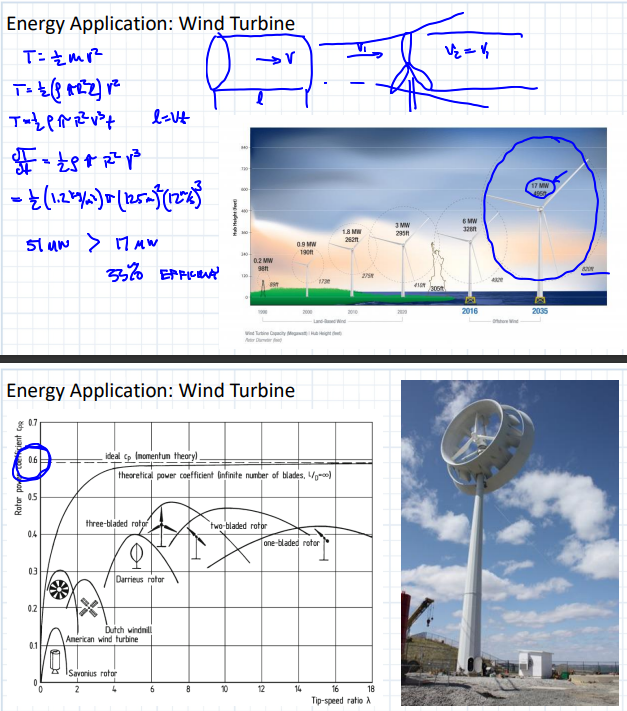
\includegraphics{WorkEnergyFigs/AppWindTurbine.png}
    \caption{From L29-Notes, slides 11-12}
    \label{fig:AppWindTurbine}
    \end{figure}
    
    
    \subsubsection{\red{Race Cars}}
    \red{This is included in L33-Notes, slides 11-12. Include the information in Fig \ref{fig:AppRaceCars}.} Application for "Friction".
    
    \begin{figure}[h!]
    \centering 
    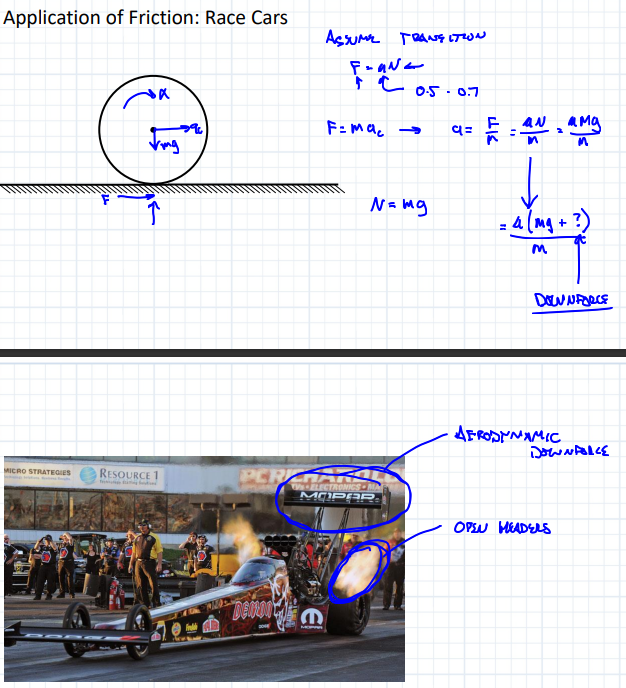
\includegraphics{WorkEnergyFigs/AppRaceCars.png}
    \caption{From L33-Notes, slides 11-12}
    \label{fig:AppRaceCars}
    \end{figure}